\documentclass{scrartcl}

\usepackage{graphicx}
\usepackage[utf8]{inputenc}
\usepackage[T1]{fontenc}
\usepackage{lmodern}
\usepackage[english]{babel}
\usepackage{amsmath}
\usepackage{amsthm}
\usepackage{mathtools}
\usepackage{amssymb}
\usepackage{listings}
\usepackage{xparse}
\usepackage{stmaryrd}
\usepackage{geometry}
\usepackage{enumerate}
\usepackage{tikz}
\usepackage{stmaryrd}
\usepackage[style=english]{csquotes}
\usepackage[language=english, backend=biber, style=alphabetic, sorting=nyt]{biblatex}

\usetikzlibrary{babel, positioning, shapes.geometric, arrows, arrows.meta}
\addbibresource{../bibliography.bib}
\title{Generating supersingular curves with modular polynomials}
\author{Simon Pohmann}

\newcommand{\Z}{\mathbb{Z}}
\newcommand{\Q}{\mathbb{Q}}
\newcommand{\F}{\mathbb{F}}
\newcommand{\C}{\mathbb{C}}
\newcommand{\End}{\mathrm{End}}
\newcommand{\Quot}{\mathrm{Quot}}
\newcommand{\Half}{\mathcal{H}}
\newcommand{\Lattice}{\mathcal{L}}
\newcommand{\divides}{\ \mid \ }
\newcommand{\notdivides}{\ \nmid \ }
\newcommand{\Cl}{\mathrm{Cl}}
\newcommand{\q}{\mathfrak{q}}
\newcommand{\Norm}{\mathfrak{N}}
\newcommand{\IdPoint}{O}
\renewcommand{\l}{\mathfrak{l}}
\renewcommand{\a}{\mathfrak{a}}
\newcommand{\p}{\mathfrak{p}}
\renewcommand{\b}{\mathfrak{b}}
\newcommand{\val}{v}
\newcommand{\Ell}{\mathrm{Ell}}
\renewcommand{\O}{\mathcal{O}}

\newcommand\restr[2]{{
    \left.\kern-\nulldelimiterspace
    #1
    \vphantom{\big|}
    \right|_{#2}
}}

\newtheorem{prop}{Proposition}[section]
\newtheorem{theorem}[prop]{Theorem}
\newtheorem{lemma}[prop]{Lemma}
\newtheorem{corollary}[prop]{Corollary}

\theoremstyle{definition}
\newtheorem{problem}[prop]{Problem}
\newtheorem{alg}[prop]{Algorithm}
\newtheorem{definition}[prop]{Definition}
\newtheorem{example}[prop]{Example}
\newtheorem{remark}[prop]{Remark}

\begin{document}

\maketitle

\section{Introduction}

\section{Ordinary isogeny graphs}

\begin{definition}
    For an integral ideal $\a \leq \End(E)$ of an ordinary Elliptic Curve $E$, define the $\a$-torsion
    \begin{equation*}
        E[\a] := \bigcap_{\alpha \in \a} \ker(\alpha)
    \end{equation*}
\end{definition}
\begin{lemma}
    Let $\phi: E \to E'$ be an isogeny.
    Then there is an isomorphism
    \begin{equation*}
        \Phi: \End(E) \otimes \Q \to \End(E') \to \Q, \quad \tau \mapsto \frac 1 {\deg(\phi)} \phi \circ \tau \circ \hat{\phi}
    \end{equation*}
    Furthermore, if we assume $E$ to be ordinary, then this is canonical in the sense that for any other isogeny $\psi: E \to E'$ have $\Phi = \Psi$.
\end{lemma}
\begin{prop}
    Let $\phi: E \to E'$ be an isogeny of prime degree $p$.
    Then (after embedding $\End(E')$ via $\Phi$ and $\End(E)$ into $\End(E) \otimes \Q$) exactly one of the following is the case.
    \begin{itemize}
        \item $\End(E) = \End(E')$ and we call $\phi$ \emph{horizontal}.
        \item $\End(E) \subseteq \End(E')$ with $[\End(E') : \End(E)] = p$. We call $\phi$ \emph{ascending}.
        \item $\End(E) \supseteq \End(E')$ with $[\End(E) : \End(E')] = p$. We call $\phi$ \emph{descending}.
    \end{itemize}
\end{prop}
\begin{prop}
    Similarly, let $\phi: E \to E'$ be an isogeny of any degree $n$.
    Further, let $l$ be a prime.
    Then (after embedding $\End(E') \otimes \Z_{(l)}$ via $\Phi$ and $\End(E) \otimes \Z_{(l)}$ into $\End(E) \otimes \Q$)exactly one of the following is the case.
    \begin{itemize}
        \item $\End(E) \otimes \Z_{(l)} = \End(E') \otimes \Z_{(l)}$ and we call $\phi$ \emph{horizontal at $l$}.
        \item $\End(E) \otimes \Z_{(l)} \subseteq \End(E') \otimes \Z_{(l)}$ with $[\End(E') \otimes \Z_{(l)} : \End(E) \otimes \Z_{(l)}] = l^r$ for $r > 0$. We call $\phi$ \emph{ascending at $l$}.
        \item $\End(E) \otimes \Z_{(l)} \supseteq \End(E') \otimes \Z_{(l)}$ with $[\End(E) \otimes \Z_{(l)} : \End(E') \otimes \Z_{(l)}] = p$ for $r > 0$. We call $\phi$ \emph{descending at $l$}.
    \end{itemize}
\end{prop}
\begin{definition}
    For an ordinary Elliptic Curve $E$ and an integral, invertible ideal $\a = \b(p, \pi_E)^r \leq \End(E)$ with $\b \perp (p, \pi_E)$ define the isogeny
    \begin{equation*}
        \phi_{E, \a}: E \ \longrightarrow \ E/E[\b] \ \overset{\pi}{\longrightarrow} \ E_\a := (E/E[\b])^{(p^r)}
    \end{equation*}
    where $E \to E/E[\b]$ is the separable isogeny with kernel $E[\b]$ and $\pi: E/E[\b] \to (E/E[\b])^{(p^r)}$ is the $r$-th power Frobenius map.
\end{definition}
\begin{lemma}
    Let $E$ be an ordinary Elliptic Curve and $\a \leq \End(E)$ an integral, invertible ideal.
    Then $\End(E) \cong \End(E_\a)$.
    In particular, $\phi_{E, \a}$ is horizontal at every prime $l$.
\end{lemma}
\begin{proof}
    Let $\a = \b(p, \pi_E)^r$ with $\b \perp (p, \pi_E)$.
    We show that $\End(E) \cong \End(E/E[\b])$ and the claim follows, as for any Elliptic Curve $E$, have an isomorphism
    \begin{equation*}
        \End(E) \to \End(E^{(p)}), \quad \alpha \mapsto \alpha^{(p)}
    \end{equation*}
    It suffices to show that the isogeny $\phi: E \to E' := E/E[\b]$ is horizontal at each prime $l$.

    Assume for a contradiction that $\phi$ is descending at $l$.
    In other words, there is $\tau \in \End(E)$ such that $\phi \circ \tau \circ \hat{\phi}$ is not divisible by $l$.
    Hence, $E'[l] \not\subseteq \ker(\phi \circ \tau \circ \hat{\phi})$ and there is a point $P \in E'[l]$ with $\phi(\tau(\hat{\phi}(P))) \neq \IdPoint$.
    This implies $\tau(\hat{\phi}(P)) \notin E[\a]$ and thus there is $\alpha \in \a$ with $\tau(\hat{\phi}(P)) \notin \ker(\alpha)$.
    Note that $\alpha$ factors through $\phi$ as
    \begin{center}
        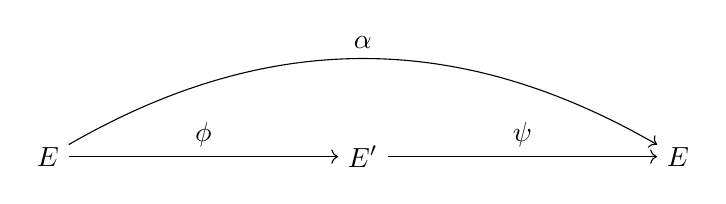
\begin{tikzpicture}
            \node (Ep) at (0, 0) {$E'$};
            \node (E1) at (-4, 0) {$E$};
            \node (E2) at (4, 0) {$E$};

            \draw [->] (E1) -- (Ep) node [midway, above] {$\phi$};
            \draw [->] (Ep) -- (E2) node [midway, above] {$\psi$};
            \draw [->] (E1) to [bend left] node [midway, above] {$\alpha$} (E2);
        \end{tikzpicture}
    \end{center}
    We assume $l \divides n$, otherwise the claim is trivial.
    However, then we have the contradiction
    \begin{align*}
        \psi((\phi \circ \tau \circ \hat{\phi})(P)) &= (\psi \circ \phi \circ \tau \circ \hat{\phi})(P) = (\alpha \circ \tau \circ \hat{\phi})(P) \\
        &= (\tau \circ \alpha \circ \hat{\phi})(P) = (\tau \circ \psi \circ [n])(P) = (\tau \circ \psi)(\IdPoint) = \IdPoint
    \end{align*}
    since $\tau \circ \alpha = \alpha \circ \tau$ ($\End(E)$ is commutative).
\end{proof}
\begin{lemma}
    Let $\O$ be a quadratic imaginary order with $p \notdivides d(\O)$ with two integral, invertible ideals $\a, \b \leq \O$.
    Let further $E$ be an Elliptic Curve with $\End(E) \cong \O$.
    Identifying $\End(E_\a)$ with $\O$ by the canonical isomorphism $\Phi_{E, \a}: \End(E) \overset{\sim}{\longrightarrow} \End(E_\a)$, we have
    \begin{equation*}
        E_{\a\b} \cong (E_\a)_\b \quad \text{and} \quad \phi_{E, \a\b} = \phi_{E_\a, \b} \circ \phi_{E, \a}
    \end{equation*}
\end{lemma}
\begin{proof}
    First, we show that $\Phi_{E, \a}(\pi_E) = \pi_{E_\a}$ and so we can write $\pi \in \O$ for the unique element mapping to the Frobenius in $\End(E)$ resp. $\End(E_\a)$.
    We have that
    \begin{equation*}
        \Phi_{E, \a}(\pi_E) = \frac 1 {\deg(\phi_{E, \a})} \phi_{E, \a} \circ \pi_E \circ \hat{\phi}_{E, \a}
    \end{equation*}
    and so
    \begin{equation*}
        \phi_{E, \a} \circ \hat{\phi}_{E, \a} \circ \Phi_{E, \a}(\pi_E) = \phi_{E, \a} \circ \pi_E \circ \hat{\phi}_{E, \a}
    \end{equation*}
    Counting separability degrees on both sides shows that $\Phi_{E, \a}(\pi_E)$ is purely inseparable, thus must be the Frobenius $\pi_{E_\a}$.
    
    Now write $\a = \tilde{\a} (p, \pi)^r$ and $\b = \tilde{\b} (p, \pi)^s$.
    It is now the case that
    \begin{equation*}
        \phi_{E, \a\b} = \phi_{E, \tilde{\a} \tilde{\b}}^{(p^{r + s})}
    \end{equation*}
    and
    \begin{equation*}
        \phi_{E_\a, \b} \circ \phi_{E, \a} = (\phi_{E_\a, \tilde{\b}} \circ \pi_r \circ \phi_{E, \tilde{\a}})^{(p^s)} = (\phi_{E_\a, \tilde{\b}} \circ \phi)^{(p^r)} = (\phi_{E_\a, \tilde{\b}}^{(q/p^r)} \circ \phi_{E, \tilde{\a}})^{(p^{r + s})}
    \end{equation*}
    where $\pi_r: E_{\tilde{\a}} \to E_{\tilde{\a}}^{(p^r)}$ is the $r$-th power Frobenius and $\phi_{E_\a, \tilde{\b}}$ is defined over $\F_q$.
    Note that $\phi_{E_\a, \tilde{\b}}$ is the separable isogeny with kernel $E_\a[\tilde{\b}]$ and thus $\phi_{E_\a, \tilde{\b}}^{(q/p^r)}$ is the separable isogeny with kernel $E_{\a}^{(q/p^r)}[\tilde{\b}] = E_{\tilde{\a}}[\tilde{\b}]$.
    In other words, find
    \begin{equation*}
        \phi_{E_\a, \tilde{\b}}^{(q/p^r)} = \phi_{E_{\tilde{\a}}, \tilde{\b}}
    \end{equation*}
    and so it suffices to show the claim in the case that $\a = \tilde{\a}$, $\b = \tilde{\b}$ are integral, invertible ideals coprime to $(p, \pi)$.

    Having reduced everything to the separable case, it now suffices to show that $\ker(\phi_{E_\a, \b} \circ \phi_{E, \a}) = E[\a\b]$.
    For simplicity of notation, write $\phi = \phi_{E, \a}$ and $\psi = \phi_{E_\a, \b}$.
    Hence, we want to show that $\ker(\psi \circ \phi) = E[\a\b]$.

    The crucial point here is that our isomorphism $\End(E) \cong \End(E_\a)$ is given by $\Phi$.
    Since the identification of $\End(E)$ and $\End(E_\a)$ would hide this, we will be explicit in this part and write
    \begin{align*}
        i: \O \to \End(E) \quad \text{and} \quad i': \O \to \End(E')
    \end{align*}
    for the isomorphisms.
    Note that $\Phi \circ i = i'$.
    We have
    \begin{align*}
        \ker(\psi \circ \phi) =& \phi^{-1}(\ker\psi) = \phi^{-1}(E'[\mathfrak{a}]) = \phi^{-1}\Bigl( \bigcap_{\tau \in \mathfrak{a}} \ker(i'(\tau)) \Bigr) \\
        =& \bigcap_{\tau \in \mathfrak{a}} \phi^{-1}(\ker(i'(\tau))) = \bigcap_{\tau \in \mathfrak{a}} \ker(i'(\tau) \circ \phi) \overset{(*)}{=} \bigcap_{\tau \in \mathfrak{a}} \ker(\phi \circ i(\tau)) \\
        =& \bigcap_{\tau \in \mathfrak{a}} i(\tau)^{-1}(\ker\phi) = \bigcap_{\tau \in \mathfrak{a}} i(\tau)^{-1}(E[\mathfrak{b}]) = \bigcap_{\tau \in \mathfrak{a}, \ \rho \in \mathfrak{b}} i(\tau)^{-1}(\ker(i(\rho))) \\
        =& \bigcap_{\tau \in \mathfrak{a}, \ \rho \in \mathfrak{b}} \ker(\underbrace{i(\rho) \circ i(\tau)}_{\mathclap{= i(\rho\tau) \in i(\a\b)}}) = E[\mathfrak{b}\mathfrak{a}]
    \end{align*}
    The equality at $(*)$ holds, since
    \begin{equation*}
        i'(\tau) = (\Phi_* \circ i)(\tau) = \frac 1 {\deg(\phi)} \phi \circ i(\tau) \circ \hat{\phi} \qedhere
    \end{equation*}
\end{proof}
\begin{lemma}
    Let $E$ be an ordinary curve and $\a, \b \leq \End(E)$ two integral, invertible ideals.
    Then $E_\a \cong E_\b$ if and only if $[\a] = [\b] \in \Cl(\End(E))$ are in the same ideal class.
\end{lemma}
\begin{theorem}
    Let $\O$ be an imaginary quadratic order with $p \notdivides d(\O)$ and denote by $\Ell(\O)$ the set of isomorphism classes of all Elliptic Curves $E$ over $\bar{\F}_p$ with $\End(E) \cong \O$.
    Then there is a free and transitive group action
    \begin{equation*}
        \Cl(\O) \times \Ell(\O) \to \Ell(\O), \quad ([\a], E) \mapsto E_\a
    \end{equation*}
    where $\a$ is an integral, invertible ideal representative of the ideal class $[\a]$.
\end{theorem}

\section{Supersingular isogeny graphs}

\section{Generating supersingular curves}

\end{document}
